% !TEX options=--shell-escape
\documentclass [12pt]{article} 

\usepackage {amsmath}
\usepackage {amsthm}
\usepackage {amssymb}
\usepackage {graphicx} 
\usepackage {float}
\usepackage {multirow}
\usepackage {xcolor}
\usepackage {algorithmic}
\usepackage [ruled,vlined,commentsnumbered,titlenotnumbered]{algorithm2e} \usepackage {array} 
\usepackage {booktabs} 
\usepackage {url} 
\usepackage {parskip} 
\usepackage [margin=1in]{geometry} 
\usepackage [T1]{fontenc} 
\usepackage {cmbright} 
\usepackage [many]{tcolorbox} 
\usepackage [colorlinks = true,
            linkcolor = blue,
            urlcolor  = blue,
            citecolor = blue,
            anchorcolor = blue]{hyperref} 
\usepackage {enumitem} 
\usepackage {xparse} 
\usepackage {verbatim}
\usepackage{listings}
\usepackage{xcolor}
\usepackage{csquotes}
\usepackage[cache=false]{minted}
\usepackage{mdframed}
\usepackage{tikz}
\usetikzlibrary{shapes.symbols}
\newtheorem{theorem}{Theorem}

\BeforeBeginEnvironment{minted}{\begin{mdframed}}
\AfterEndEnvironment{minted}{\end{mdframed}}

\DeclareTColorBox {Solution}{}{breakable, title={Solution}}
\DeclareTColorBox {Solution*}{}{breakable, title={Solution (provided)}}
\DeclareTColorBox {Instruction}{}{boxrule=0pt, boxsep=0pt, left=0.5em, right=0.5em, top=0.5em, bottom=0.5em, arc=0pt, toprule=1pt, bottomrule=1pt}
\DeclareDocumentCommand {\Expecting }{+m}{\textbf {[We are expecting:} #1\textbf {]}}
\DeclareDocumentCommand {\Points }{m}{\textbf {(#1 pt.)}} 
\newcommand {\hint }[1]{\noindent {[\textbf {HINT:} \em #1 \em ]}} \newcommand {\pts }[1]{\textbf {(#1 pt.)}} 

\begin{document} 

{\LARGE \textbf {COMP 285 (NC A\&T, Spr `22)}\hfill \textbf {Homework 6} } 
\vspace {1em} 
\begin{Instruction} 

\paragraph {Due.} Wednesday, February 23rd, 2022 @ 11:59 PM!
\end{Instruction} 

\vspace {1em} 
\begin{Instruction} \paragraph {Homework Expectations:} Please see \href{https://www.comp285.ml/homework/#general-homework-information}{Homework}.
\end{Instruction}

\vspace {1em} 
\begin{Instruction} 

\paragraph {Exercises} The following questions are exercises. We encourage you to work with a group and discuss solutions to make sure you understand the material.

\paragraph {Points} This assignment is graded out of 100 points. However, you can get up to 120 points if you complete everything. These are not bonus points, but rather points to help make-up any parts you miss.

\end{Instruction} 

\begin{centering}
\section*{Fun with TOOD}
\end{centering}

\begin{Instruction}

\paragraph{Written Problems} The following questions are to be submitted in written/typed form to gradescope.

\end{Instruction}

\section{Interview Practice: DFS Basics \Points{10}}
\label{sec:last}

Consider the following directed acyclic graph (DAG): 

\begin{center}
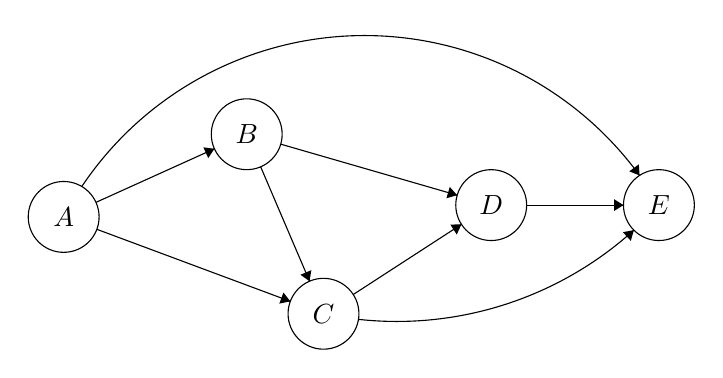
\begin{tikzpicture}[scale=0.15] 
    \tikzstyle{every node}+=[inner sep=0pt]
    \draw [black] (18.2,-24.6) circle (3);
    \draw (18.2,-24.6) node {$A$}; 
    \draw [black] (33.7,-17.6) circle (3);
    \draw (33.7,-17.6) node {$B$};
    \draw [black] (40.2,-32.8) circle (3);
    \draw (40.2,-32.8) node {$C$};
    \draw [black] (54.4,-23.6) circle (3);
    \draw (54.4,-23.6) node {$D$};
    \draw [black] (68.6,-23.6) circle (3);
    \draw (68.6,-23.6) node {$E$};
    \draw [black] (57.4,-23.6) -- (65.6,-23.6);
    \fill [black] (65.6,-23.6) -- (64.8,-23.1) -- (64.8,-24.1);
    \draw [black] (20.93,-23.37) -- (30.97,-18.83);
    \fill [black] (30.97,-18.83) -- (30.03,-18.71) -- (30.44,-19.62);
    \draw [black] (34.88,-20.36) -- (39.02,-30.04);
    \fill [black] (39.02,-30.04) -- (39.17,-29.11) -- (38.25,-29.5);
    \draw [black] (42.72,-31.17) -- (51.88,-25.23);
    \fill [black] (51.88,-25.23) -- (50.94,-25.25) -- (51.48,-26.09);
    \draw [black] (21.01,-25.65) -- (37.39,-31.75);
    \fill [black] (37.39,-31.75) -- (36.81,-31) -- (36.46,-31.94);
    \draw [black] (36.58,-18.44) -- (51.52,-22.76);
    \fill [black] (51.52,-22.76) -- (50.89,-22.06) -- (50.61,-23.02);
    \draw [black] (19.736,-22.025) arc (146.19641:36.07693:28.811);
    \fill [black] (66.96,-21.09) -- (66.9,-20.15) -- (66.09,-20.74);
    \draw [black] (66.48,-25.721) arc (-47.8655:-96.2357:29.916);
    \fill [black] (66.48,-25.72) -- (65.55,-25.89) -- (66.22,-26.63);
\end{tikzpicture} 
\end{center} 

In class, we saw how to use DFS to find a topological ordering of the the vertices; in the graph above, the unique topological ordering is $A,B,C,D,E$. We saw an example where we happened to start DFS from the first vertex in the topological order. In this exercise we'll see what happens when we start at a different vertex. Recall that when you run DFS, if it reached a node with no children (i.e. can’t go any further), then it will resume the search at an unvisited vertex. 


\subsection {\Points {5}} 

Run DFS starting at vertex $C$, breaking any ties by alphabetical order.\footnote {For example, if DFS has a choice between $B$ or $C$, it will always choose $B$. This includes when DFS is starting a new tree in the DFS forest.}

\begin{enumerate}[label=(\alph *)]
    \item What do you get when you order the vertices by \textbf {ascending} start time?
    \item What do you get when you order the vertices by \textbf {descending} finish time?
\end{enumerate} 

\subsection {\Points {5}}

Run DFS starting at vertex $C$, breaking any ties by \textbf {reverse} alphabetical order.\footnote {For example, when DFS has a choice between $B$ or $C$, it will always choose $C$. This includes when DFS is starting a new tree in the DFS forest.}

\begin{enumerate}[label=(\alph *)]
    \item What do you get when you order the vertices by \textbf {ascending} start time?
    \item What do you get when you order the vertices by \textbf {descending} finish time?
\end{enumerate} 

\Expecting {For all four questions, an ordering of vertices. No justification is required.} 

\begin{Instruction}

\paragraph{Coding Problems} The following questions are to be submitted as a ".zip" file on Gradescope. 

\end{Instruction}

\section{Coding \Points{50}}
After completing the written portion of the assignment, you should submit it to \href{https://www.gradescope.com/courses/350304}{Gradescope}.

For the coding portion, tou can get your starter code \href{https://replit.com/team/COMP285/HW5-Code}{here}.

Note that the starter code also include a few test cases you can run on repl.it. However, the full test suite is the one run on Gradescope.

Please reference the \texttt{README.md} included in your starter code for detailed instructions.

\section*{Submitting the Assignment}

This assignment is a combination of written and programming questions. Both portions of the assignment should be submitted through \href{https://www.gradescope.com/courses/350304}{Gradescope}.

The "Homework 6: Fun with " assignment is the written portion, for which you should submit a \textbf{typed} response to the non-coding questions (questions 1-\ref{sec:last}). Each response should clearly be marked with its corresponding number. You are free to use the provided templates, print the questions and write your answers, or to simply type your responses on a blank document (whatever works for you).

The "Homework 6: Coding" is the programming portion of the assignment. For this portion, download the ".zip" file from replit and upload this ".zip" file as your answer to \href{https://www.gradescope.com/courses/350304}{Gradescope}. You can upload the assignment as many times as you want.


\end{document} 